% Overleaf source revision: completed-results-20260917
\documentclass{article} % For LaTeX2e
\usepackage[T1]{fontenc}
\usepackage{iclr2027_conference,times}

\newcommand{\siqi}[1]{\textcolor{blue}{[siqi: #1]}}

% ------------------------------ Preamble ------------------------------------
\usepackage{graphicx}
\usepackage{float}
\usepackage{placeins}
\usepackage{array}
\usepackage{booktabs}
\usepackage{xcolor}
\newfloat{algorithm}{t}{loa}
\floatname{algorithm}{Algorithm}

\usepackage{amsmath,amssymb,mathtools,bm}
\usepackage{amsthm}

\newtheorem{definition}{Definition}
\newtheorem{lemma}{Lemma}
\newtheorem{proposition}{Proposition}
\newtheorem{theorem}{Theorem}
\newtheorem{corollary}{Corollary}
\theoremstyle{remark}
\newtheorem{remark}{Remark}

% Visible author annotations replace incomplete experimental figures and tables.
\newcommand{\completionnote}[2]{%
  \par\smallskip\noindent
  \fcolorbox{blue!35!black}{blue!3}{%
    \parbox{\dimexpr\linewidth-2\fboxsep-2\fboxrule\relax}{%
      \small\textbf{To complete: #1.} #2}}%
  \par\smallskip}

\newcommand{\cD}{\mathcal{D}}
\newcommand{\cV}{\mathcal{V}}
\newcommand{\sg}{\operatorname{sg}}
\newcommand{\norm}[1]{\left\lVert #1 \right\rVert}
\newcommand{\inner}[2]{\left\langle #1,#2 \right\rangle}
\newcommand{\pospart}[1]{\left[#1\right]_{+}}
\newcommand{\ctr}[2]{\operatorname{ctr}_{#1}\!\left[#2\right]}
\newcommand{\chisq}[2]{\chi^2\!\left(#1\,\|\,#2\right)}
% Optional math commands from https://github.com/goodfeli/dlbook_notation.
\input{math_commands.tex}

\usepackage{hyperref}
% Keep the template default hyperlink borders (citations green, internal links red).
\hypersetup{
    pdftitle={Token Balancing, Update Sparsity, and Supervision Density in Multi-Teacher On-Policy Distillation},
    pdfauthor={Anonymous Authors}}
\usepackage{url}


\title{Understanding Multi-Teacher On-Policy Distillation: From Gradients to Capabilities}

\author{Anonymous Authors}


%\iclrfinalcopy
\begin{document}


\maketitle

\begin{abstract}

Multi-teacher on-policy distillation (MOPD) trains a single student using specialized teachers, but the effects of loss normalization, vocabulary supervision, and optimizer dynamics on parameter updates and task performance are not well understood. We study these effects with a Qwen3-1.7B student and four teachers for mathematics, code, instruction following, and science. First, averaging losses over tokens rather than responses changes gradient directions even when total loss weights are equal between domains. Nevertheless, three normalization rules differ by only 0.14 percentage points in final mean score under student--teacher top-64 intersection supervision with Adam. Second, after 500 updates, training changes about 97\% of FP32 master weights but only 7.3--8.5\% of stored BF16 weights. Teacher-specific Adam updates appear aligned largely because they use the same accumulated moment estimates: subtracting the update that Adam would take with no new gradient reduces their mean cosine similarity from above 0.83 to below 0.01 on domain-specific inputs. Third, the intersection of the student's and teacher's top-64 token sets contains over 99.9\% of student probability mass on average at the evaluated checkpoints, and expanding supervision to the full vocabulary barely changes single-step update concentration. Yet we find no consistent performance advantage for top-64 over sampled-token supervision: at the joint-training endpoint, mathematics increases by 2.60 points while GPQA decreases by 1.77 points, with both paired 95\% confidence intervals including zero. Thus sparse BF16 changes do not imply sparse optimization, and aligned Adam updates do not imply aligned teacher gradients. Neither statistic can replace per-task evaluation when choosing a distillation objective.

\end{abstract}

\section{Introduction}
\label{sec:intro}

Multi-teacher on-policy distillation (MOPD) is used in LLM post-training to transfer specialized capabilities into a single model \citep{xiaomi2026mimov2flash,nvidia2026nemotron3ultra,kimiteam2026kimik3openfrontier,deepseekai2026deepseekv4highlyefficientmilliontoken}. The student generates responses, and a teacher assigned to each prompt domain supplies token-level supervision. The training objective is to improve several capabilities while preserving the student's existing performance. Achieving this requires deciding how much each domain and response contributes to the loss, and how many next-token alternatives the teacher supervises.

Recent work establishes both the potential of MOPD and the sensitivity of its results to these choices. \citet{ma2026mopdmultiteacheronpolicydistillation} study capability integration with policy-gradient and top-$k$ distillation objectives. Open-MOPD finds uneven transfer between domains and introduces domain token balancing, weighting by student--teacher performance gaps, and refreshed rewards \citep{gao2026openmopddiagnosingfixingcapability}. The Nemotron 3 Ultra report finds no advantage for top-$k$ or full-vocabulary matching over sampled-token supervision in its preliminary experiments \citep[Section~3.3.5]{nvidia2026nemotron3ultra}. Studies of OPD parameter changes also report concentration in a small set of stored weights \citep{yu2026denseupdates,shen2026opdgeometry}. These findings leave open how the loss weights and vocabulary targets affect the gradients, optimizer updates, and task scores of a jointly trained student.

Three distinctions matter for answering this question. First, equal numbers of prompts per domain do not imply equal domain contributions to a token-averaged loss, because response lengths differ. Even after fixing each domain's total loss weight, averaging over tokens or over responses gives different weights to long responses. Second, Adam updates depend on accumulated first- and second-moment estimates as well as the current gradient, and small FP32 updates may disappear when weights are stored in BF16. Sparse stored-weight changes or similar Adam update directions can therefore reflect the optimizer and numerical precision. Third, supervising more vocabulary tokens need not improve every task, even when the resulting parameter updates have similar concentration.

We study these distinctions through training runs and controlled gradient and optimizer comparisons with Qwen3-1.7B and four domain teachers. The main findings are:
\begin{enumerate}
\item \textbf{Different normalization rules produce distinct gradients but similar final top-64/Adam scores (Section~\ref{sec:normalization}).}
With equal prompt counts, mathematics receives 44.05\% of the token-averaged loss weight and instruction following 14.98\%. Fixing domain weights does not remove response-length weighting: token and response averaging have a mean gradient cosine of 0.680. Applying the same Adam moment estimates raises their update cosine to 0.960. The three normalization rules finish within 0.14 mean-score points under top-64 supervision, although their learning curves differ; sampled-token/SGD runs have a larger 1.07-point spread.
\item \textbf{BF16 sparsity and Adam update alignment can obscure the current teacher gradient (Section~\ref{sec:subnetworks}).}
Joint training changes about 97\% of FP32 master weights but only 7.3--8.5\% of stored BF16 weights. At the same student checkpoint, teacher-specific Adam updates have mean cosine similarity above 0.83 on their respective domain inputs. Removing the step that Adam would take using its accumulated moments with a zero current gradient reduces the cosine below 0.01. Thus aligned optimizer steps do not establish aligned current teacher gradients.
\item \textbf{More vocabulary supervision does not consistently improve task performance (Section~\ref{sec:density}).}
Sampled-token, top-64, and full-vocabulary losses produce similarly concentrated single-step updates when the top-64 intersection already contains over 99.9\% of student probability on average. In joint training, top-64 supervision scores 2.60 points higher on mathematics and 1.77 points lower on GPQA than sampled-token supervision at update 500; all paired task intervals include zero. Its mean advantage also shrinks from 1.69 points at update 250 to 0.29 points at update 500.
\end{enumerate}

These results motivate evaluating supervision choices with per-task learning curves in addition to gradient and parameter statistics. Section~\ref{sec:recipe} evaluates development-selected checkpoints on separate test sets: adding a per-domain retention constraint does not change any selected checkpoint in the ten tested trajectories.

\section{Preliminaries}
\label{sec:setting}

\paragraph{Multi-teacher on-policy distillation (MOPD).}
For domain $d$, the student generates $y\sim p_\theta(\cdot\mid x)$ for $x\sim\mathcal D_d$, and a frozen teacher $q_d$ supplies probabilities at each prefix $h_t=(x,y_{<t})$ \citep{gao2026openmopddiagnosingfixingcapability}. For a rollout batch $\mathcal B$, response $i$ has $T_i$ valid tokens and mean loss $\ell_i=T_i^{-1}\sum_t\ell_{i,t}$. The objective is
\begin{equation}
\mathcal L(\theta)=\sum_{i\in\mathcal B}w_i\ell_i(\theta),
\qquad w_i\geq0,\quad\sum_{i\in\mathcal B}w_i=1.
\label{eq:mopd}
\end{equation}
The token loss determines the vocabulary supervision; the response weights $w_i$ determine normalization across tokens, responses, and domains. Each update uses fresh student responses, held fixed with their masks and weights during gradient computation.

\paragraph{Sampled-token, top-$k$, and full-vocabulary supervision.}
Write $p_\theta(v)=p_\theta(v\mid h_t)$ and $q_d(v)=q_d(v\mid h_t)$. Full-vocabulary supervision minimizes reverse KL over $\mathcal V$; the policy-gradient (PG) loss scores the sampled token $y_t$:
\begin{equation}
\label{eq:full}
\ell_{\mathrm{full}}=\sum_{v\in\mathcal V}p_\theta(v)\log\frac{p_\theta(v)}{q_d(v)},\qquad
\ell_{\mathrm{PG}}(y_t)=-\sg[\log q_d(y_t)-\log p_\theta(y_t)]\log p_\theta(y_t)
\end{equation}

Here $\sg$ denotes stop-gradient. At a fixed prefix, the expected PG gradient equals the full reverse-KL gradient: differentiating Equation~\ref{eq:full} gives $\sum_v[\log(p_\theta(v)/q_d(v))+1]\nabla_\theta p_\theta(v)$. The $+1$ term cancels because $\sum_v\nabla_\theta p_\theta(v)=0$, leaving $\mathbb E_{a\sim p_\theta}[\log(p_\theta(a)/q_d(a))\nabla_\theta\log p_\theta(a)]$.

Top-$k$ supervision uses $I=S\cap T$, where $S,T$ are the student and teacher top-$k$ sets, computed at rollout and held fixed. Its loss is
\begin{equation}
\ell_{\mathrm{top}\text{-}k}=-\sum_{v\in I}\sg\!\left[
\frac{p_\theta(v)}{\sum_{u\in S}p_\theta(u)}
\bigl(\log q_d(v)-\log p_\theta(v)\bigr)\right]\log p_\theta(v).
\label{eq:topk}
\end{equation}
Probabilities use the full-vocabulary softmax; detached weights are normalized over $S$, and an empty intersection gives zero loss. We call the number of supervised vocabulary tokens the \emph{supervision density}: one for PG, $|I|\leq k$ for intersection supervision, and $|\mathcal V|$ for full supervision.

\paragraph{Intersection supervision is a biased gradient surrogate.}
For a fixed set $A$, write $Z_A=\sum_{v\in A}p_\theta(v)$ and $g_A=\sum_{v\in A}\log(p_\theta(v)/q_d(v))\nabla_\theta p_\theta(v)$. Unlike the full-vocabulary cancellation, $\nabla_\theta Z_I$ is generally nonzero. Thus directly truncating the KL objective gives $\nabla_\theta\sum_{v\in I}p_\theta(v)\log(p_\theta(v)/q_d(v))=g_I+\nabla_\theta Z_I$. Equation~\ref{eq:topk} instead uses detached coefficients, so its gradient and discrepancy from full KL are
\begin{equation}
\nabla_\theta\ell_{\mathrm{top}\text{-}k}=\frac{g_I}{Z_S},\qquad
\nabla_\theta\ell_{\mathrm{top}\text{-}k}-\nabla_\theta\ell_{\mathrm{full}}
=\left(\frac{1}{Z_S}-1\right)g_I-g_{\mathcal V\setminus I}.
\label{eq:intersection_bias}
\end{equation}
I64 therefore omits contributions outside $I$ and rescales those retained by $1/Z_S$; it is neither an unbiased full-KL gradient estimator nor the gradient of the directly truncated KL objective. The missing $+1$ term follows from stop-gradient, not cancellation on $I$. These differences mean that PG--I64 comparisons change the gradient surrogate as well as supervision density.

\paragraph{Domain weighting and loss normalization.}
Let $\mathcal B_d$ contain responses from domain $d$, and let $\lambda_d\geq0$ with $\sum_d\lambda_d=1$ be the target domain loss weights. For nonempty responses and domains, the three rules assign response $i\in\mathcal B_d$ weights
\begin{equation}
w_i^{\mathrm{GT}}=\frac{T_i}{\sum_{j\in\mathcal B}T_j},\qquad
w_i^{\mathrm{DT}}=\frac{\lambda_d T_i}{\sum_{j\in\mathcal B_d}T_j},\qquad
w_i^{\mathrm{DR}}=\frac{\lambda_d}{|\mathcal B_d|}.
\label{eq:averaging}
\end{equation}
Global-token (GT) averaging weights domains by their response-token shares. Domain-token (DT) and domain-response (DR) averaging fix each domain's total weight to $\lambda_d$: DT weights responses by length, while DR weights their mean losses equally. Domain loss weights are distinct from prompt sampling proportions.

\paragraph{Update similarity.}
Let $u_d$ be the parameter change from one step on domain $d$'s mean loss. Each compared step starts from identical student weights and optimizer state, including Adam's moments. For nonzero updates, their cosine is $C_{de}=(u_d^\top u_e)/(\|u_d\|\,\|u_e\|)$.

\section{Loss Normalization and Task Performance}
\label{sec:normalization}

\subsection{Equal domain weights do not remove response-length weighting}

Sampling equal numbers of prompts per domain does not give each domain equal weight in the training loss, because student response lengths differ by domain. With token-level normalization over the full batch (GT), domains with longer responses receive more loss weight. Domain-token normalization (DT) fixes each domain's weight to $\lambda_d$ but still assigns longer responses more weight within that domain. Domain-response normalization (DR) also fixes the domain weights and gives equal weight to each response's mean loss. Domain balancing and within-domain loss normalization are therefore separate design choices, even with a fixed prompt mixture.

This difference changes the gradient whenever response length correlates with the response gradient. Write $g_i=\nabla_\theta\ell_i$, and let $\bar g_d$ and $\bar T_d$ denote the mean response gradient and response length within domain $d$. The token-weighted domain gradient satisfies
\begin{equation}
\frac{\sum_{i\in\mathcal B_d}T_i g_i}{\sum_{i\in\mathcal B_d}T_i}
=\bar g_d+\frac{\operatorname{Cov}_d(T,g)}{\bar T_d}.
\label{eq:weighting}
\end{equation}
The covariance term measures the effect of weighting response gradients by length. DT retains this term; DR uses $\bar g_d$ alone. Multiplying each domain's GT loss contribution by its target weight $\lambda_d$ divided by its observed token share gives DT exactly, as in Open-MOPD \citep[Section~4.1, Eq.~(8)]{gao2026openmopddiagnosingfixingcapability}. Thus correcting unequal domain token counts still leaves a choice between token-level and sequence-level normalization within each domain. Appendix~\ref{app:normalization} gives the derivation.

\subsection{Similar I64 endpoint scores despite different loss weights}

\paragraph{Training and evaluation.}
We train a Qwen3-1.7B student with four frozen teachers for mathematics, code, instruction following, and science. The three I64 configurations differ only in GT, DT, or DR loss normalization. They use the same initialization, teachers, prompt schedule, and optimizer settings, with 16 prompts per domain at each update. We evaluate MATH-500, a fixed LiveCodeBench subset, IFBench, and GPQA Diamond through update 500 and report their equally weighted mean. Appendix~\ref{app:setup} gives the training and scoring protocol.

\paragraph{Correcting a threefold loss-weight imbalance changes little at the I64 endpoint.}
Mathematics and instruction following each receive 25\% of prompts but account for 44.05\% and 14.98\% of GT's valid response tokens in the first 50 batches. GT therefore assigns mathematics nearly three times as much loss weight as instruction following, whereas DT and DR fix both at 25\% (Figure~\ref{fig:normalization_capability}a). Despite this difference, the update-500 four-domain scores are $38.58\pm0.75$\% (DR), $38.71\pm0.80$\% (DT), and $38.64\pm0.80$\% (GT), reported as mean $\pm$ standard deviation over three training seeds. The 0.14-percentage-point range between means is smaller than the 0.75--0.80-point seed standard deviations. The preferred rule varies with the task and checkpoint: all three improve mathematics and instruction following toward teacher performance, retain a code performance gap, and start near the science teacher's GPQA score (Figure~\ref{fig:normalization_capability}). Equal domain loss weights therefore do not consistently improve the final mean score in this I64/Adam setting.

\begin{figure}[t]
\centering
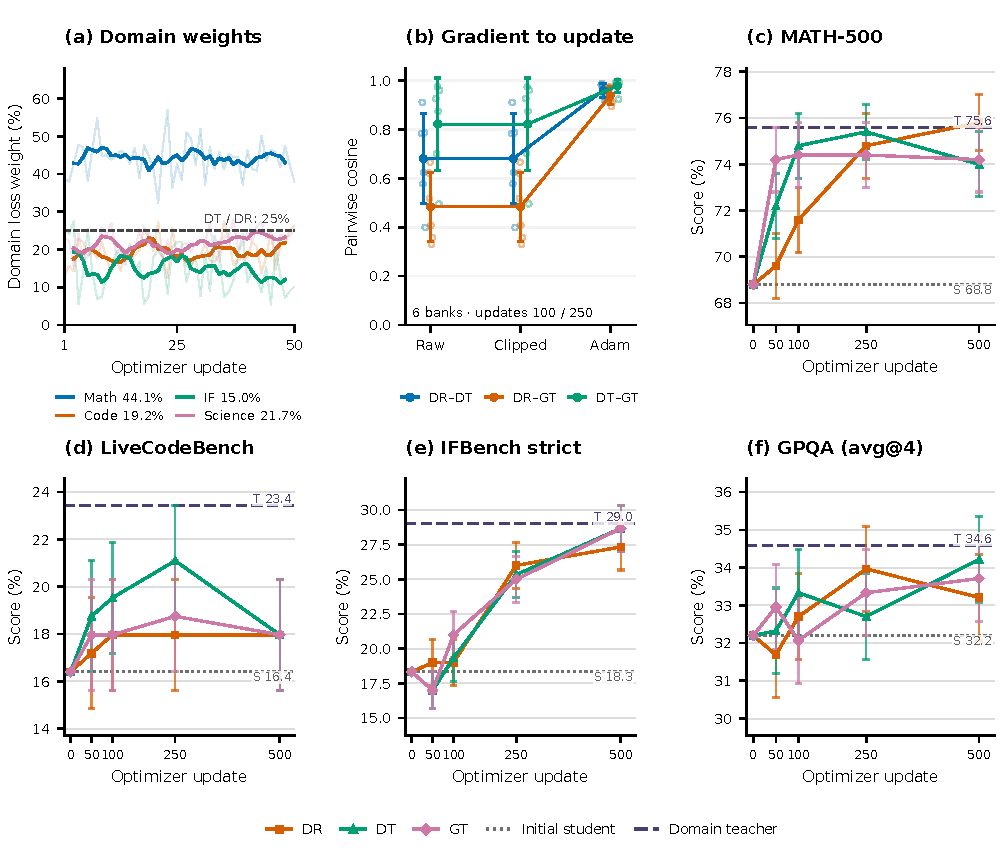
\includegraphics[width=\linewidth]{figures/nine_panel_20260914/section3_normalization.pdf}
\caption{Loss weighting, optimizer mediation, and task capability trajectories.
(a) GT domain loss weights across the first 50 updates: faint lines are individual batches, bold lines are five-batch moving averages, and legend values are arithmetic means over all 50 batches. DT and DR each fix domain weights at 25\%.
(b) Three reduction pairs before clipping, after clipping, and after a shared saved-state Adam update. Small open points are six fixed banks at updates 100/250; lines and error bars show their mean and sample standard deviation.
(c--f) GT/DT/DR scores on MATH-500, LiveCodeBench, IFBench strict, and GPQA (avg@4), with initial-student (S) and domain-teacher (T) references. Points and error bars retain the original means and sample standard deviations, computed from measured seed-42 scores and estimated seed-43/44 scores. The authors report agreement with subsequent three-seed experiments; the retained estimates are not independently verified measurements. Updates use a linear axis. Appendix Figure~\ref{fig:normalization_aggregate_support} gives the four-domain mean and worst-domain change.}
\label{fig:normalization_capability}
\end{figure}


\paragraph{Normalization changes PG/SGD endpoint scores by 1.07 points.}
In the seed-42 endpoint comparison, the four-domain score range between normalization rules is 0.33 points for PG/Adam and 1.07 points for PG/SGD, compared with 0.14 points for I64/Adam (Table~\ref{tab:completed_endpoints}). PG/SGD favors DR over GT by 1.07 points, while PG/Adam favors GT over DR by 0.07 points. The small differences under I64/Adam therefore do not establish that normalization is unimportant for other training configurations. All ten configurations improve the initial four-domain mean from 33.93\% to 38.03--39.46\%. These results use one training seed, unlike the three-seed I64 summary above. The SGD runs also use a different learning rate and deployment, so their higher scores do not isolate the effect of the optimizer or establish a training-efficiency advantage. Appendix~\ref{app:completed_results} reports the separate test-set evaluation.

% Estimated paired intervals: experiments/table1_paired_estimates_20260918/estimate_intervals.py.
\begin{table}[t]
\centering\small
\setlength{\tabcolsep}{3.5pt}
\caption{\textbf{Task gains coexist with domain-level trade-offs.} Joint-training endpoint scores (\%); Mean weights domains equally. PG: sampled-token supervision; I16/I64: top-16/top-64 intersection supervision. DR/DT: equal domain weights with response/token averaging; GT: global token averaging. $\Delta$ is the mean difference from PG-DR/Adam (percentage points). Brackets give model-based paired 95\% intervals (Appendix~\ref{app:capability_uncertainty}).}
\label{tab:completed_endpoints}
\begin{tabular}{lrrrrrr}
\toprule
Configuration & MATH-500 & Code & IF & GPQA & Mean & $\Delta$ [95\% interval] \\
\midrule
Initial student & 68.80 & 16.41 & 18.33 & 32.20 & 33.94 & $-4.68$ [-6.42, -2.93] \\
\midrule
\multicolumn{7}{l}{\textit{Adam}} \\
PG-DR & 73.20 & 18.27 & 27.00 & 35.97 & 38.61 & Reference \\
PG-DT & 73.20 & 19.24 & 27.00 & 34.96 & 38.60 & $-0.01$ [-1.45, 1.43] \\
PG-GT & 76.20 & 17.92 & 27.33 & 32.94 & 38.60 & $-0.01$ [-1.44, 1.42] \\
I16-DR & 75.40 & 17.75 & 27.00 & 35.46 & 38.90 & $+0.29$ [-1.15, 1.73] \\
I64-DR & 75.80 & 18.30 & 27.33 & 34.71 & 39.04 & $+0.43$ [-1.01, 1.86] \\
I64-DT & 74.00 & 18.86 & 28.67 & 35.22 & 39.19 & $+0.58$ [-0.87, 2.02] \\
I64-GT & 74.20 & 19.80 & 28.67 & 33.41 & 39.02 & $+0.41$ [-1.03, 1.85] \\
\midrule
\multicolumn{7}{l}{\textit{SGD}} \\
PG-DR & 76.40 & 19.53 & 28.33 & 35.59 & 39.96 & $+1.35$ [-0.09, 2.79] \\
PG-DT & 75.20 & 20.31 & 28.33 & 33.90 & 39.44 & $+0.83$ [-0.61, 2.26] \\
PG-GT & 75.00 & 19.26 & 25.33 & 34.71 & 38.58 & $-0.04$ [-1.47, 1.40] \\
\bottomrule
\end{tabular}
\par\vspace{2pt}
\end{table}


\subsection{Adam reduces directional differences between normalization rules}

\paragraph{Different gradients produce more similar Adam updates.}
I64 gradient cosines average 0.680 (DR--DT), 0.483 (DR--GT), and 0.822 (DT--GT) on six fixed response batches at joint-PG checkpoints 100 and 250. These comparisons hold the student weights, responses, token masks, and teacher scores fixed, so the directional differences come from loss normalization. In particular, the DR--DT comparison shows that equal domain weights do not eliminate the effect of response-length weighting. Applying each gradient from an identical copy of the saved Adam first- and second-moment estimates raises the corresponding FP32 update cosines to 0.960, 0.939, and 0.979. The resulting parameter updates are therefore much more similar in direction than the gradients used to compute them.

\paragraph{Gradient clipping changes magnitude, not direction.}
Global norm clipping leaves all three pairwise gradient cosines unchanged. Its frequency nevertheless differs sharply during training: DR is clipped on all 500 updates and retains a median 9.3\% of the gradient norm, whereas DT and GT are clipped on 46.2\% and 15.0\% of updates, respectively (Figure~\ref{fig:normalization_interventions}a). Clipping alone therefore cannot explain the increase in update cosine under Adam. Resetting Adam's moment estimates also changes the update norms (Figure~\ref{fig:normalization_interventions}b), showing that the saved optimizer state affects update magnitude as well as direction.

\paragraph{One-step loss changes also depend on the optimizer state.}
After one Adam step from the same saved moment estimates, the three normalization rules produce similar changes in held-out reverse KL relative to the variation between response batches (Figure~\ref{fig:normalization_interventions}c). When SGD steps are rescaled to match each rule's Adam update norm, the differences between rules are larger: all three reduce mean held-out KL at update 100 but increase it at update 250. These measurements concern the immediate effect of one update on fixed held-out responses. They do not account for the complete training trajectories, in which each student generates different responses and accumulates different Adam moments. Appendix~\ref{app:fixed_batch_normalization} gives the one-step protocol and gradient comparisons; Figure~\ref{fig:normalization_ci} reports paired task-score contrasts.

\begin{figure}[t]
\centering
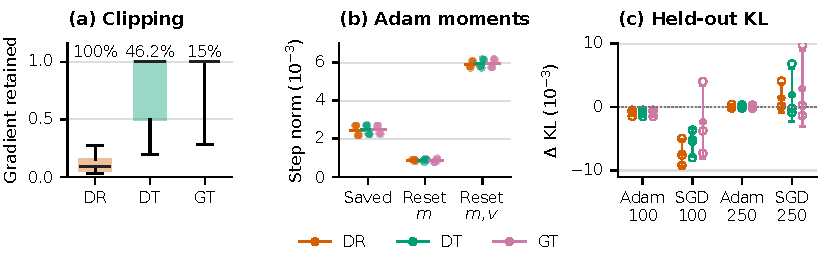
\includegraphics[width=\linewidth]{figures/added_control_figures_20260914/normalization_interventions.pdf}
\caption{Optimizer interventions.
(a) Gradient fraction retained over 500 updates per reduction; labels give clipping rates, boxes the interquartile range, and whiskers the 5th--95th percentiles.
(b) FP32 step norms across six banks; bars show means.
(c) Immediate held-out reverse-KL changes under saved Adam and norm-matched SGD; lower is better. Open points denote banks; filled points and error bars show mean $\pm$ sample SD.}
\label{fig:normalization_interventions}
\end{figure}


\FloatBarrier

\section{Update Sparsity and Teacher Overlap}
\label{sec:subnetworks}

This study examines how numerical representation and optimizer history affect the concentration, overlap, and direction of teacher-conditioned parameter changes. Prior work observes concentrated changes under dense distillation supervision \citep{yu2026denseupdates}. We examine the corresponding measurements in a jointly trained student.

\subsection{How concentrated are joint parameter changes?}

Write $\Delta=\theta-\theta_0$ for cumulative changes from initialization and $u=\theta_{\mathrm{after}}-\theta_{\mathrm{before}}$ for an individual optimizer step. For either change vector $z$ with $P$ coordinates, we report the fraction of parameters whose absolute change exceeds threshold $\tau$:
\begin{equation}
 f_\tau(z)=\frac{1}{P}\sum_{j=1}^{P}\mathbf 1\{|z_j|>\tau\}.
 \label{eq:active_fraction}
\end{equation}
We also report the smallest coordinate fraction accounting for 90\% of the squared change. This measures concentration without choosing an absolute threshold. Both quantities are computed separately for FP32 optimizer weights and BF16 stored model weights.

\paragraph{Joint-training comparison.}
The M-PG and M-I64-DR branches share the training settings in Appendix~\ref{app:setup}, including domain-response averaging. Figure~\ref{fig:geometry} compares cumulative changes at common updates 1, 50, 100, 250, and 500. At update 250, PG changes 5.88\% of BF16 coordinates, with 90\% of squared change in 3.01\% of coordinates. I64 changes 7.13\%, with 90\% of squared change in 3.94\%. Both joint runs concentrate their stored parameter changes in a small fraction of the model.

The corresponding FP32 nonzero fractions are 95.73\% for PG and 96.07\% for I64. Their 90\%-energy fractions are 32.94\% and 34.82\%. Thus the apparent sparsity depends strongly on which parameter representation is measured. The actual optimizer steps at update 250 change 86.35\% of FP32 coordinates for PG and 86.70\% for I64. Threshold curves and optimizer-state controls appear in Appendix~\ref{app:records}.

\begin{figure}[t]
\centering
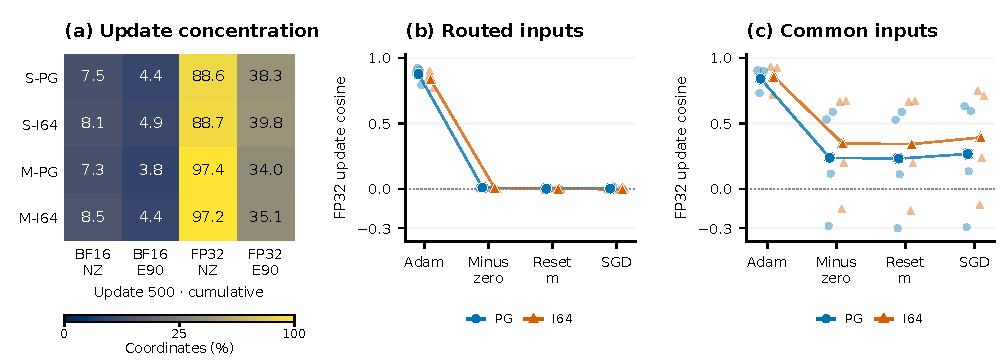
\includegraphics[width=\linewidth]{figures/nine_panel_20260914/section4_sparsity_overlap.pdf}
\caption{Parameter concentration and teacher-conditioned updates.
(a) Cumulative changes at update 500 for single-teacher (S) and joint (M) PG/I64 training, using DR. NZ is the nonzero coordinate fraction; E90 is the coordinate fraction carrying 90\% of squared change. Cells give percentages; color uses a square-root scale. S receives four times as many mathematics responses per update as M.
(b) At the common M-PG/500 student and optimizer state, FP32 top-1\% Jaccard versus signed update cosine. Small points average six teacher pairs within each bank; large points average four banks. Lines connect common-input (open) and routed-input (filled) conditions. SGD and reset-$m$ are individually norm-matched to saved-state Adam; circles denote PG and triangles I64.
(c) Teacher JS and $1-J$ on common inputs, with all six teacher pairs in all four banks. Colors and loss markers match (b); points share teachers and banks and are dependent. Updates use non-fused PyTorch steps on saved-state copies, rather than bitwise replay of the online optimizer.}
\label{fig:subnetwork_overview}
\end{figure}


\noindent Figure~\ref{fig:subnetwork_overview}(a) adds the matched single-teacher and joint cumulative measurements at update 500. The full recorded trajectories remain available in the accompanying evidence bundle.

\subsection{Do teachers change the same parameters in one student?}

Comparing teacher-specific updates requires identical copies of the joint student and its optimizer state. For teacher $d$, let $S_d(\rho)$ contain the largest-magnitude $\rho$ fraction of its parameter changes. We compare selected coordinates using Jaccard overlap:
\begin{equation}
J(d,e)=\frac{|S_d(\rho)\cap S_e(\rho)|}{|S_d(\rho)\cup S_e(\rho)|}.
\label{subnet_overlap}
\end{equation}
Equal selection sizes make the teacher pairs comparable. Overlap describes locations; the signs of the changes determine whether contributions at those locations agree. This distinction follows the support-overlap analysis of \citet{yu2026denseupdates}.

At the common M-PG/500 state, routed-input teacher updates have mean FP32 cosines of 0.8774 for PG and 0.8347 for I64 under saved-state Adam. Resetting the first moment or using norm-matched SGD brings their mean cosines close to zero (Figure~\ref{fig:subnetwork_overview}b). Each small point summarizes six teacher pairs within one of four response banks; large points average the four banks. These are local diagnostic repeats, not independent training runs. Appendix~\ref{app:completed_results} retains the joint overlap--direction and teacher-JS views, while Appendix~\ref{app:gradient_overlap} gives the separate raw-gradient input controls.

\subsection{How much alignment remains after removing the history-only step?}

Let $U(g;H)$ denote an optimizer step for current gradient $g$ at saved optimizer state $H$. We compare the complete teacher-conditioned step with its difference from the zero-current-gradient step,
\begin{equation}
\delta U_d=U(g_d;H)-U(0;H).
\label{eq:history_subtracted}
\end{equation}
This difference retains the same parameters and optimizer state in both branches. It is a nonlinear counterfactual difference, not an additive decomposition of teacher contributions.

Under routed inputs, the mean PG/I64 cosines fall to 0.0098/0.0067 after this subtraction (Figure~\ref{fig:subnetwork_overview}b). Under common inputs, they fall from 0.8415/0.8562 to 0.2373/0.3462 (panel c). The strong alignment of the complete steps therefore depends on shared optimizer history and input conditions. Routed inputs vary both teacher identity and input domain; common-input controls hold the prefixes fixed. Coordinate overlap can remain substantial even when directions differ, and neither statistic establishes the absence of cross-domain functional harm. The required teacher-by-probe-domain loss intervention is distinct from this geometric comparison.

\section{Vocabulary Supervision: Parameter Updates and Task Performance}
\label{sec:density}

Expanding supervision from one sampled token to a larger vocabulary set changes gradient approximation and task-level learning. We compare sampled-token supervision with the student--teacher top-64 intersection during mathematics-only and joint training. Full-vocabulary supervision supplies a reference for the gradient and single-step comparisons.

\subsection{Broader supervision produces task-dependent gains}

\paragraph{The mathematics advantage develops during training.}
In mathematics-only training, sampled-token supervision leads top-64 by 2.8 accuracy points at update 100; top-64 leads by 2.2 points at update 500 (Figure~\ref{fig:supervision_overview}c). Joint training also ends with a mathematics gain from top-64 supervision, accompanied by a science loss: final differences are $+2.6$ points on mathematics and $-1.2$ on GPQA. Code and instruction-following differences are smaller.

Top-64's joint-training mean advantage narrows from 1.69 points at update 250 to 0.43 at update 500. These trajectories show that the observed benefit depends on the task and the stage of training.

\paragraph{Larger candidate sets redistribute gains across tasks.}
Top-16 and top-64 supervision reach development means of 39.03\% and 39.04\%, and separate-test means of 44.56\% and 44.46\% (Table~\ref{tab:main_outcomes}). On the separate tests, top-64 gains 1.96 mathematics points and loses 2.35 code points relative to top-16.

\begin{figure}[t]
\centering
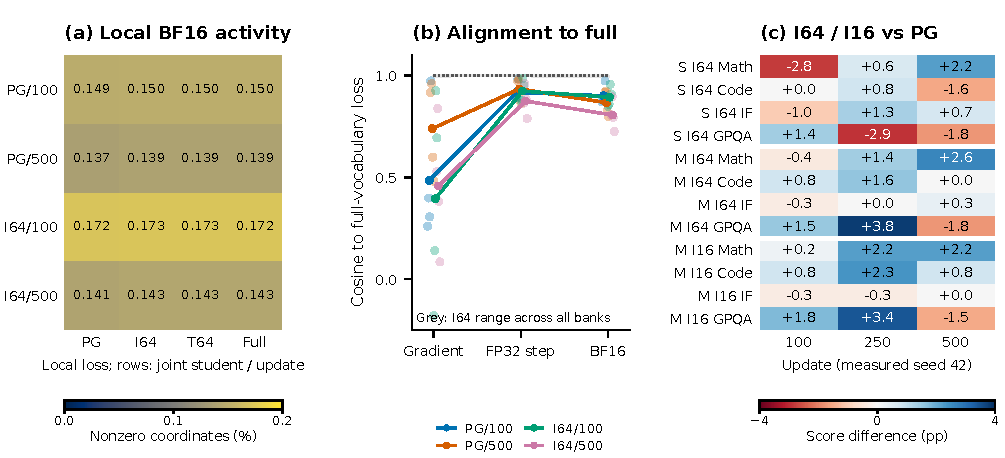
\includegraphics[width=\linewidth]{figures/nine_panel_20260914/section5_supervision.pdf}
\caption{Supervision geometry and capability.
(a) Mean BF16 nonzero fractions by student state and loss.
(b) Alignment with full-vocabulary supervision: PG bank means (lines) and individual banks (points), with the I64 range shaded.
(c) I64-minus-PG task scores (percentage points); positive values favor I64. S/M denote single-teacher/joint training.}
\label{fig:supervision_overview}
\end{figure}


\subsection{Larger candidate sets improve gradient approximation}
\label{sec:coverage_gradient}

Truncating vocabulary support omits probability mass and changes token weights \citep{anshumann2025sparse,huang2026tailaware}. We measure coverage as the student probability retained by the student--teacher candidate intersection, $c_k(h)=\sum_{v\in S\cap T}p_\theta(v\mid h)$, and compare gradients.

\paragraph{Top-64 closely matches the full-vocabulary direction in Qwen.}
The intersection retains over 99.9\% of student probability on average, and its gradient direction is close to that of full-vocabulary supervision (Figure~\ref{fig:supervision_overview}b). Averaging 1, 16, and 64 token samples raises the mean gradient cosine from 0.54 to 0.87 to 0.97; top-64 exceeds 0.999 (Figure~\ref{fig:sampling_history_controls}a). This sampling control identifies finite-sample variation as one source of the directional difference.

\paragraph{Lower-coverage inputs retain appreciable gradient error in SmolLM.}
SmolLM3-3B measurements use the MixSFT initialization and its student after 500 updates of top-64 training with response averaging and three teachers for mathematics, code, and instruction following \citep{gao2026openmopddiagnosingfixingcapability}. Mean top-64 coverage is 97.42\% initially and 98.56\% after training; 8.42\% and 3.65\% of weighted prefixes retain less than 90\% mass (Figure~\ref{fig:smollm_supervision}a,b). Larger candidate sets reduce this low-coverage tail.

We compare gradients on typical prefixes, high-entropy prefixes, and prefixes with top-64 coverage below 99\%. Top-64 has 2.16--24.54\% relative gradient error against full-vocabulary supervision. Top-4 and top-8 produce larger errors in the evaluated batches (Figure~\ref{fig:smollm_supervision}d). Here relative error is the norm of the gradient difference divided by the full-vocabulary gradient norm, capturing both direction and magnitude. Larger candidate sets improve the approximation, with residual error at top-64.

\begin{figure}[t]
\centering
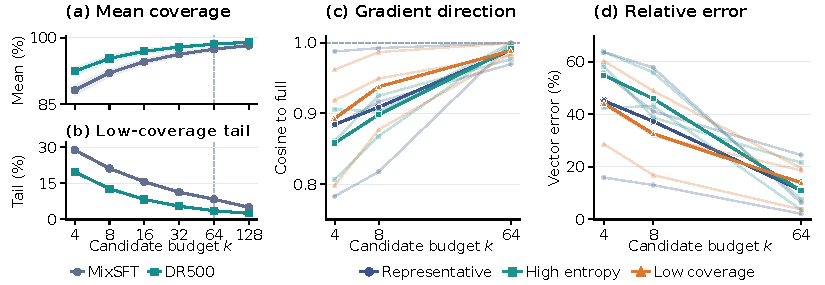
\includegraphics[width=\linewidth]{figures/layout_followup_20260918/smollm_supervision.pdf}
\caption{\textbf{Larger candidate sets improve coverage and gradient approximation in SmolLM.}
(a,b) Mean retained student probability and fraction of inputs below 90\% coverage; bands show response-cluster 95\% intervals. Dashed lines mark top-64.
(c,d) Gradient cosine and relative error against full-vocabulary supervision at the trained student. Groups comprise typical inputs, uncertain next-token predictions, and inputs with lower top-64 coverage; thin lines show batches and bold lines their means. MixSFT/DR500 denote the initialization/trained student.}
\label{fig:smollm_supervision}
\end{figure}

\paragraph{SmolLM capability scores also reveal changes below the aggregate.}
Sampled-token training with SGD raises MATH-500 accuracy from 50.60\% to 53.80\%. On AIME 2025, the initialization, the top-64/domain-token Adam student, and the sampled-token/response-averaged SGD student each solve four of 30 questions with eight samples per question; only one solved question is common to all three.


\subsection{Vocabulary supervision leaves single-step concentration nearly unchanged}

Sampled-token, top-64, teacher-top-64, and full-vocabulary losses produce nearly identical single-step concentration (Figure~\ref{fig:supervision_overview}a). This similarity across vocabulary supports is consistent with concentrated stored-weight changes under dense distillation \citep{yu2026denseupdates}.

The teacher-top-64 reference uses a fixed teacher top-64 set $T$ and full-vocabulary probabilities:
\begin{equation}
\ell_{\mathrm{T64}}=\sum_{v\in T}\left[p_\theta(v)\log\frac{p_\theta(v)}{q_d(v)}-p_\theta(v)+q_d(v)\right].
\label{eq:t64}
\end{equation}
The $-p_\theta(v)$ correction cancels the $+1$ derivative term on this restricted support; $q_d(v)$ is constant with respect to the student and makes each summand zero when $p_\theta(v)=q_d(v)$. Hence $\nabla_\theta\ell_{\mathrm{T64}}=g_T$, using the notation of Section~\ref{sec:setting}. T64 omits terms outside $T$ but has no $1/Z_S$ rescaling, whereas I64 uses $g_I/Z_S$. Neither generally recovers the full-KL gradient. T64 and full KL are single-step references; end-to-end training compares PG, I16, and I64.

Shared optimizer history contributes strongly to the similar concentration. Even a zero current gradient changes about 0.14\% of BF16 parameters in the same comparison, close to the fraction changed by the supervised losses. Resetting Adam's moments changes the amount of BF16 writeback (Figure~\ref{fig:sampling_history_controls}b,c).

\begin{figure}[t]
\centering
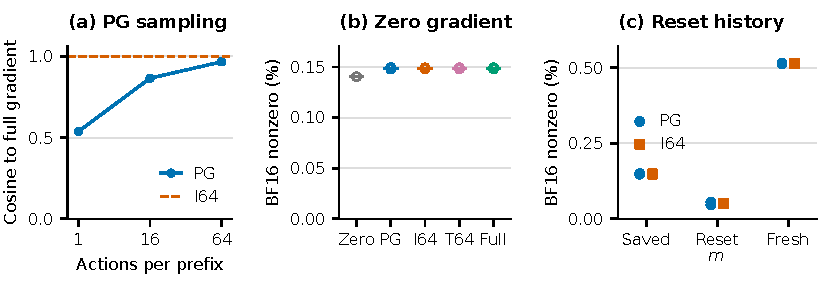
\includegraphics[width=\linewidth]{figures/added_control_figures_20260914/sampling_history_controls.pdf}
\caption{\textbf{More token samples increase PG gradient cosine to full-vocabulary KL; Adam momentum alone changes nearly as many BF16 parameters as PG.}
(a) Gradient cosine to full-vocabulary KL.
(b,c) Nonzero BF16 changes with a zero current gradient or reset Adam moments. Points denote cached batches; bars show means.}
\label{fig:sampling_history_controls}
\end{figure}


Over training, student parameters, responses, and optimizer moments evolve together. Top-64 and sampled-token supervision consequently accumulate different BF16 displacements (Section~\ref{sec:subnetworks}), alongside the task-dependent learning trajectories above.

\FloatBarrier

\section{Practical Implications and Checkpoint Selection}
\label{sec:recipe}

The three studies support practical choices about weighting, diagnostics, and evaluation. They do not identify one configuration that is best across domains and evaluation sets.

\paragraph{Specify the intended weighting and measure the resulting capability profile.}
GT weights tokens equally; DT fixes domain weights while retaining length weighting within each domain; DR also weights responses equally. These are different objectives, even with the same prompt quotas. Likewise, the PG/I16/I64 results favor selecting vocabulary feedback from per-domain capability and measured cost, with retained probability mass used to interpret coverage. The present runs do not provide a matched-cost efficiency ranking.

\paragraph{Interpret update geometry with its history and precision.}
Report the parameter representation, distinguish individual steps from cumulative changes, and compare teacher-conditioned updates at a common state. A zero-current-gradient reference helps assess how much alignment depends on shared history. Evidence of overlap or opposing directions should be followed by per-domain loss or capability measurements before inferring functional interference.

\paragraph{Evaluate checkpoint selection on separate questions.}
To test domain retention as a selection criterion, let $s_d(\theta)$ be a development score, with higher values better, and let $\epsilon_d\geq0$ be a prespecified tolerance relative to initialization. Eligible checkpoints satisfy
\begin{equation}
s_d(\theta)\geq s_d(\theta_0)-\epsilon_d
\qquad\text{for every domain }d.
\label{eq:retention}
\end{equation}
We select the eligible checkpoint with maximum equal-domain mean, retaining the initial student if none improves it by at least one percentage point. We compare this rule with unconstrained maximum utility and the final checkpoint, using a two-point domain tolerance fixed before the additional test results. Appendix~\ref{app:completed_selection} gives the development grids and selection outcomes.


The additional test uses separately frozen questions from four domain sources, with 256 questions per domain and a distinct evaluation protocol (Appendix~\ref{app:independent_domain_test}). Relative rankings can change: PG-DR/SGD exceeds Adam by 1.18 mean points on the original benchmarks, but is 0.07 points lower on this test. Retention and unconstrained maximum utility select the same checkpoint on all ten trajectories: update 500 in nine cases and update 250 for PG-DT/Adam. In the latter case, the selected checkpoint scores 43.14\% on the additional test, versus 43.51\% at update 500. The retention constraint therefore has no demonstrated selection benefit here. Because the development benchmarks had been observed previously, this selection study remains exploratory.

\section{Related Work}

\paragraph{Distillation objectives and vocabulary truncation.}
MiniLLM uses reverse KL \citep{gu2024minillm}; Generalized Knowledge Distillation (GKD) combines student-generated sequences with alternative divergences \citep{agarwal2024gkd}; $f$-DISTILL derives word-level losses from sequence-level $f$-divergences \citep{wen2023fdivergence}. Sparse Logit Sampling analyzes top-$k$ caching bias \citep{anshumann2025sparse}, while Tail-Aware OPD restores tail-mass information lost by top-$k$ renormalization \citep{huang2026tailaware}. Our intersection loss retains full-softmax log ratios with detached student-top-$k$ weights. Section~\ref{sec:density} compares its coverage, gradient error, updates, and task scores with sampled-token and full-vocabulary supervision.

\paragraph{Multi-teacher distillation and loss normalization.}
MOPD integrates specialized teachers on student-generated responses \citep{ma2026mopdmultiteacheronpolicydistillation}; Open-MOPD adds domain token balancing and adaptive weighting \citep{gao2026openmopddiagnosingfixingcapability}. DAPO uses token-level averaging \citep{yu2025dapo}, and Dr.~GRPO analyzes length and reward-normalization bias \citep{liu2025understandingr1zero}. We separate domain weighting from within-domain response weighting: Open-MOPD's token-share correction gives DT for fixed batches and domain weights, while DR also removes response-length weighting.

\paragraph{Post-training parameter geometry.}
\citet{mukherjee2025subnetworks} study small parameter subsets supporting RL fine-tuning; \citet{yu2026denseupdates} report concentrated distillation updates and overlap between separately trained students. \citet{shen2026opdgeometry} examine OPD geometry and response-position selection. We examine teacher alignment, distinguish FP32 from BF16 changes, and vary vocabulary support.

\section{Discussion}

The experiments use one Qwen3-1.7B student and four teachers derived from its initial model. The normalization capability summaries report seeds 42--44; the expanded objective/optimizer matrix and additional-domain test use seed 42. Local banks are diagnostic repeats, and question-bootstrap intervals measure evaluation uncertainty at fixed checkpoints. Neither substitutes for independent training runs. The local supervision comparisons also have high candidate coverage, limiting what they establish about vocabulary tails or less similar teachers. Appendix~\ref{app:math_overlap_sensitivity} reports sensitivity to four known overlapping mathematics questions; this does not constitute exhaustive decontamination.

Local update geometry and long-term capability transfer remain distinct measurements. Fixed-state interventions reveal how weighting, history, and precision affect an update; online and additional-domain evaluations establish the resulting capability trade-offs. Together they support conditional guidance for MOPD design, while broader claims about stability or efficiency require repeated training under matched budgets.

\newpage
\section*{AI use statement}
We used a large language model for minor editorial assistance, including correcting grammar and typo and refining formatting. It did not contribute to the development of research ideas, the analysis, or the claims.

\section*{Ethics Statement}
We ensure that the dataset used in this study is free from discrimination, bias, exploitation, human rights violations, and any other ethical concerns.

\section*{Reproducibility Statement}
To ensure reproducibility of our results, we provide detailed documentation of our experimental setup and methodology in the main paper and appendix. The code for data, evaluation,
and analysis will be open-sourced upon publication.



% \clearpage
\bibliography{iclr2027_conference}
\bibliographystyle{iclr2027_conference}

\clearpage
\appendix

\section{Experimental Protocol and Results}
\label{app:setup}

\subsection{Model, data, and training protocol}

The main-study student is Qwen3-1.7B \citep{qwen2025qwen3}; training uses seeds 42, 43, and 44. The four teachers were trained by reinforcement learning from the same initial model, specializing in mathematics, code, instruction following, and science, respectively.

AdamW configurations use learning rate $2.5\times10^{-7}$ with $(\beta_1,\beta_2)=(0.9,0.98)$, $\epsilon=10^{-8}$, no weight decay or schedule, and global norm-1 clipping. For the SGD runs, the learning-rate is $2.5\times10^{-2}$, following the empirically optimal setting reported by \citep{mukherjee2026sgd} analysis of AdamW's effective per-parameter learning rates and an SGD learning-rate sweep. Training sampling uses temperature 1 and top-$p=1$, with a 2,048-token prompt cap and 4,096-token response cap. One fresh response is sampled per prompt. Each optimizer update aggregates 64 responses; domain allocation is specified below.

The multi-teacher setup allocates 16 prompts to each domain per update and uses target domain weights $0.25$. The single-teacher setup allocates all 64 prompts to the same domain. I64 uses the top-$64$ objective in Equation~\ref{eq:topk}; I16 uses $k=16$.

\subsection{Evaluation and scoring}

Each main-study capability suite contains MATH-500 (500 questions) \citep{hendrycks2021math}, LiveCodeBench v6 (1,055 questions) \citep{jain2024livecodebench}, IFBench strict (300 questions) \citep{pyatkin2025ifbench}, and GPQA Diamond (198 questions) \citep{rein2023gpqa}. Mathematics, code, and instruction following use one greedy response per question. GPQA uses four responses per question at temperature 1 and top-$p=1$. Its score is the mean correctness over all four responses, then over questions: average@4 accuracy. Evaluation permits up to 32,768 response tokens, bounded by the remaining configured 32,768-token context. Each complete suite contains 2,053 questions and 2,647 responses per model evaluation.

The expanded development grid comprises updates of 50/100/250/500 for seven Adam trajectories and 100/250/500 for three SGD trajectories, plus the initial student evaluation. Appendix~\ref{app:independent_domain_test} describes additional test sets for the same four domains. Table~\ref{tab:main_outcomes} gives the complete joint-training endpoint scores. Figure~\ref{fig:supervision_overview}(c) compares single-teacher and joint-training trajectories.

The four RL teachers were evaluated separately on their respective domain benchmarks using the same prompt and decoding protocol. These scores quantify each teacher's performance on its target domain.


\section{Length-Weighting Derivation}
\label{app:normalization}

Fix a rollout batch, its valid-token masks, and domain weights $\lambda_d$. Any PG coefficients are detached. For $n_d=|\mathcal B_d|$, let $\bar T_d=n_d^{-1}\sum_{i\in\mathcal B_d}T_i$ and $\bar g_d=n_d^{-1}\sum_{i\in\mathcal B_d}g_i$. Define the empirical covariance using the same $1/n_d$ normalization:
\begin{equation}
\operatorname{Cov}_d(T,g)=\frac{1}{n_d}\sum_{i\in\mathcal B_d}(T_i-\bar T_d)(g_i-\bar g_d).
\end{equation}
Expanding gives $n_d^{-1}\sum_iT_i g_i-\bar T_d\bar g_d$. Dividing by $\bar T_d$ yields Equation~\ref{eq:weighting}. GT combines the resulting domain gradients using observed token shares; DT combines them using $\lambda_d$; DR combines $\bar g_d$ using $\lambda_d$. Multiplying each domain's globally averaged terms by its target weight divided by its observed token share therefore gives DT exactly.

The derivation is a finite-batch weighted-average identity. Response sampling, masks, and lengths are held fixed. Its population analogue involves an expectation of a ratio; replacing that expectation by a ratio of expectations requires additional assumptions or a large-batch limit.

\subsection{Fixed-batch gradient comparison}
\label{app:fixed_batch_normalization}

At M-PG checkpoints 100 and 250, three banks (seeds 1042, 1043, and 1044) each contain eight responses per domain. Responses use the training prompt format and 4,096-token response cap. For each bank, we compute each response's mean I64 gradient once at the saved BF16 model values using FP32 computation, then aggregate those gradients under DR, DT, and GT. All three reductions use the same responses, token masks, teacher scores, and model coordinates. Student and optimizer snapshots match within each checkpoint.

Table~\ref{tab:fixed_batch_normalization} reports every pairwise raw-gradient cosine. The domain-wise covariance decomposition is checked in FP64 over all 24 bank-domain groups; the largest relative residual is $1.53\times10^{-15}$. This numerical check verifies the aggregation identity. The observed gradient directions establish that the covariance contribution is nonzero on these batches.

The optimizer interventions in Figure~\ref{fig:normalization_interventions} reuse these six banks. Each aggregate gradient is globally clipped at norm 1 and applied to the same saved FP32 Adam state for that bank. The saved-state branch retains both moments; the reset-$m$ branch zeros the first moment while retaining the second moment and optimizer clock; reset-$(m,v)$ zeros both moments while retaining the clock. The momentum-free SGD control follows the negative gradient and is rescaled separately for DR, DT, and GT to match that reduction's saved-state Adam FP32 step norm. Every proposed FP32 step is cast to BF16 before evaluating one held-out response per domain. We report full-vocabulary reverse KL for evaluation; the training-consistent I64 surrogate is retained in the source bundle. These are immediate local interventions, not additional online training runs.

\begin{table}[t]
\caption{Fixed-batch averaging comparison. Entries are raw-gradient cosines; each row uses one shared student and response bank. DR and DT share domain weights and differ only in within-domain response weighting.}
\label{tab:fixed_batch_normalization}
\centering\small
\begin{tabular}{rrrrr}
\toprule
Updates & Batch & DR--DT & DR--GT & DT--GT \\
\midrule
100 & 1 & 0.7838 & 0.6219 & 0.9266 \\
100 & 2 & 0.9110 & 0.5180 & 0.7010 \\
100 & 3 & 0.5780 & 0.6659 & 0.9745 \\
250 & 1 & 0.6240 & 0.4072 & 0.8742 \\
250 & 2 & 0.7864 & 0.3302 & 0.4953 \\
250 & 3 & 0.3990 & 0.3569 & 0.9612 \\
\bottomrule
\end{tabular}

\end{table}

\section{Parameter and Optimizer Measurements}
\label{app:records}

\subsection{Coordinates and recorded quantities}

The online record distinguishes raw aggregate gradients, clipped gradients, actual FP32 optimizer steps, cumulative FP32 master changes, and cumulative BF16 model changes. Cumulative changes use the same initialization reference. All global statistics use unique model coordinates, excluding vocabulary padding and shared duplicates. Per-layer statistics and absolute-threshold sensitivities are retained in the frozen measurements. The sparsity value is the fraction at or below a threshold; figures report its complement. Energy concentration uses squared Euclidean norm and ranks coordinates by absolute change.

For local calculations, the exported checkpoint contains FP32 master values, BF16 model values, first and second moments, optimizer hyperparameters, and step clocks. Student and teacher values are verified against their saved models in the same precision. Local forward/backward computations evaluate these values in FP32 with TF32 disabled. All proposed steps are computed from the same saved state with a non-fused Adam implementation. The online training optimizer uses its own fused implementation.

We evaluate three local states. \emph{Saved} retains both moments and the step clock. \emph{Reset m} zeros the first moment while retaining the second moment and clock. \emph{Fresh} zeros both moments and resets the clock. Global norm clipping at 1 is applied before the Adam calculation, and weight decay is zero. The plotted controls use two response banks; the zero-gradient control is evaluated once. For the zero-gradient branch, the saved first moment continues to decay and move the master weights. A no-step master-to-BF16 cast gives an exact match to the saved model. Figure~\ref{fig:thresholds} shows how absolute thresholds change the measured local activity.

The zero-current-gradient branch changes 0.1403\% of BF16 coordinates, compared with 0.1486\% for PG. Resetting the first moment gives 0.0504\% for PG; resetting both moments and the clock gives 0.5140\%. These controls explain why a sparse gradient selection cannot by itself identify the parameters changed by an optimizer step. They supplement the update-sparsity measurements in Sections~\ref{sec:subnetworks} and~\ref{sec:density}.

Figure~\ref{fig:sampling_history_controls}(b,c) displays these BF16 controls. The full FP32 and BF16 measurements are retained in the evidence bundle.

\begin{figure}[t]
\centering
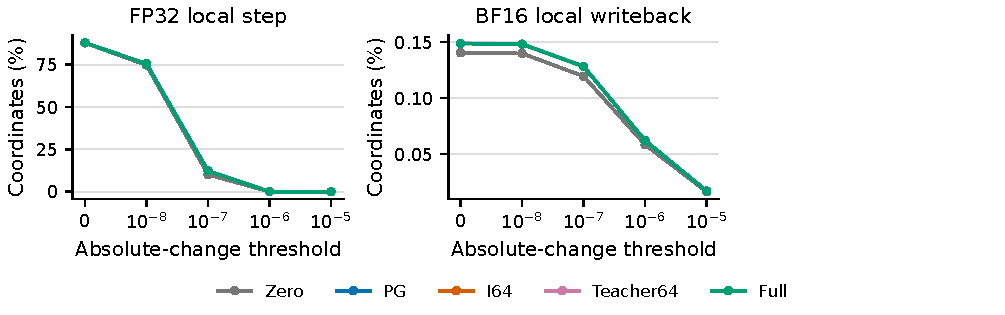
\includegraphics[width=\linewidth]{figures/aligned_evidence_20260910/thresholds.pdf}
\caption{Threshold sensitivity of FP32 steps and BF16 changes. Lines show bank means; shading spans their range.}
\label{fig:thresholds}
\end{figure}

\subsection{Response banks, overlaps, and gradient magnitudes}
\label{app:gradient_overlap}

These raw-gradient diagnostics use the M-PG/100 student, whereas Figure~\ref{fig:subnetwork_overview}(b,c) measures teacher-conditioned optimizer steps at M-PG/500. Banks use seeds 42 and 43, one response per domain per bank, a 2,048-token prompt cap, and a 256-token generation cap. All eight responses reach the cap. Four response positions are sampled without replacement per response. Each row's four prefixes receive equal weight. For routed gradients, each teacher scores its domain row; for common-bank gradients, it scores all four rows with equal domain weights. Crossed comparisons score every domain row with every teacher, keeping the number of prefixes per gradient at four. Crossed and routed/common comparisons share underlying gradients and form paired conditions within banks.

Top-$k$ coordinate sets rank absolute gradient values, using a stable coordinate index to break cutoff ties. Table~\ref{tab:coverage_mass} supplies the routed PG norms; the first bank's instruction-following gradient has norm $1.53\times10^{-9}$. Cosine normalizes magnitude, so opposite directions for such a row carry very little absolute gradient mass. Jaccard overlap measures selected locations and cosine measures signed direction. For reference, independent uniform sets of fraction $\rho$ have expected-intersection to expected-union ratio $\rho/(2-\rho)$, or approximately 0.00503 at $\rho=1\%$. This reference uses uniform coordinates; layer and weight-magnitude structure remain in the measured gradients.

Applying Equation~\ref{subnet_overlap} to the largest-magnitude 1\% of raw-gradient coordinates gives mean routed Jaccard overlaps of 0.0951 for PG and 0.0999 for I64 across the two banks and six teacher pairs. Their ranges are 0.0744--0.1077 and 0.0737--0.1178. When every teacher instead scores all four domain responses, the respective means are 0.3808 and 0.4577. The latter comparison changes both input composition and prefix count; the crossed input control below fixes the count.

Holding the teacher fixed while changing the input domain yields mean gradient cosines of 0.0059 for PG and 0.0072 for I64. Holding the input domain fixed while changing teachers produces both aligned and opposed gradients. For routed gradients the mean cosines are $-0.0020$ and $0.0081$, respectively, despite partial coordinate overlap. Figure~\ref{fig:teacher} supplies this input and direction context for the teacher-overlap results in Section~\ref{sec:subnetworks}.

\begin{figure}[t]
\centering
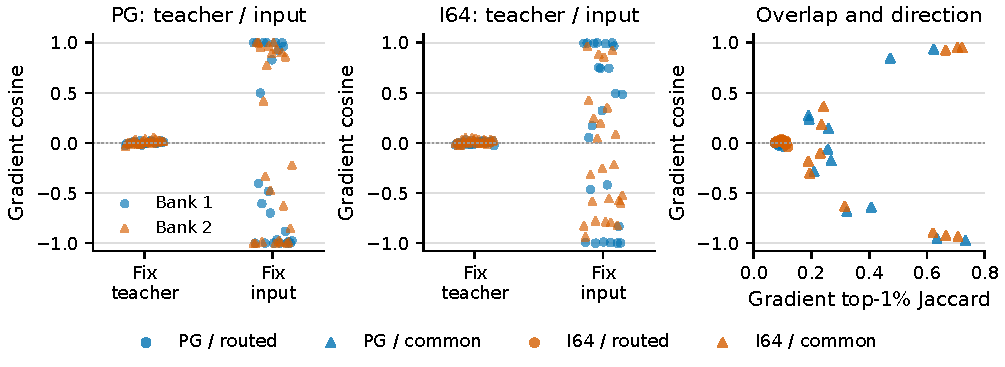
\includegraphics[width=\linewidth]{figures/aligned_evidence_20260910/teacher_input.pdf}
\caption{Input dependence of teacher overlap. Left/center: crossed teacher--input comparisons. Right: top-1\% gradient Jaccard versus signed cosine for routed and common inputs.}
\label{fig:teacher}
\end{figure}

\section{Vocabulary Supervision and Coverage}
\label{app:losses}

\paragraph{Four-bank local experiment.}
The M-PG/100 row of Figure~\ref{fig:supervision_overview}(a) uses four response banks with seeds 2042--2045. Each bank contains one response per domain. Generation uses the training prompt format, a 2,048-token prompt cap, and a 4,096-token response cap. The 16 response lengths range from 81 to 4,096 tokens; two responses reach the cap. Six positions per response give 96 prefixes. PG actions are freshly sampled from the student at the cached prefixes. Every loss uses the same prefixes and domain-response weights. Gradients are globally clipped at norm 1 before applying the same saved Adam state. Table~\ref{tab:local_concentration} adds the FP32 and energy-concentration measurements for this state.

\begin{table}[t]
\centering\small
\caption{Local concentration at M-PG/100, averaged over four matched banks. NZ is the percentage of nonzero coordinates; top-1\% is the percentage of squared step norm carried by the largest 1\% of coordinates. These are local bank means, not training-seed estimates.}
\label{tab:local_concentration}
\begin{tabular}{lrrrr}
\toprule
Loss & FP32 NZ & BF16 NZ & FP32 top-1\% & BF16 top-1\% \\
\midrule
PG & 87.982 & 0.149 & 8.845 & 100.000 \\
I64 & 87.989 & 0.150 & 8.827 & 100.000 \\
T64 & 87.989 & 0.150 & 8.828 & 100.000 \\
Full & 87.999 & 0.150 & 8.828 & 100.000 \\
\bottomrule
\end{tabular}

\end{table}

The local loss and Adam implementations are the same as in the two-bank controls in Appendix~\ref{app:records}. Appendix~\ref{app:actual_intersection_coverage} reports the actual I64 intersection coverage across all four student states.


\paragraph{Implementation details.}
For I64 (Equation~\ref{eq:topk}), candidate sets and teacher scores are fixed at rollout. Each student forward recomputes current probabilities at the saved candidate positions and refreshes the detached coefficients. PG also refreshes its detached log-ratio coefficients and uses no advantage or policy-ratio clipping.

\paragraph{Teacher-top-64 local reference.}
The teacher-top-64 diagnostic uses the fixed teacher set $T$ and full-vocabulary probabilities:
\begin{equation}
\ell_{\mathrm{T64}}=\sum_{v\in T}\left[p_\theta(v)\log\frac{p_\theta(v)}{q_d(v)}-p_\theta(v)+q_d(v)\right].
\label{eq:t64}
\end{equation}
Its gradient is $\sum_{v\in T}p_\theta(v)\log(p_\theta(v)/q_d(v))\nabla_\theta\log p_\theta(v)$. I64 instead uses the detached weights in Equation~\ref{eq:topk}, normalized over the original student set $S$. T64 and full vocabulary are local objective comparisons; online capability curves compare PG, I16, and I64. I16 has no corresponding local geometry measurement.

For a fixed prefix, differentiating Equation~\ref{eq:full} gives
\begin{align}
\nabla_\theta\ell_{\mathrm{full}}
&=\sum_{v\in\cV}p_\theta(v)\left(\log\frac{p_\theta(v)}{q_d(v)}+1\right)\nabla_\theta\log p_\theta(v)\\
&=\mathbb E_{a\sim p_\theta}\!\left[\log\frac{p_\theta(a)}{q_d(a)}\nabla_\theta\log p_\theta(a)\right],
\end{align}
using $\sum_v\nabla_\theta p_\theta(v)=0$. The identity conditions on prefixes and fixed weights. Original rollout losses additionally use the realized response and its eventual length-dependent weight. Table~\ref{tab:coverage_mass} reports the corresponding coverage for the two-bank controls used to interpret gradient overlap and optimizer history.

\begin{table}[t]
\caption{Teacher-top-64 coverage and routed gradient scale in the two-bank controls. Probability mass and student entropy (nats) are prefix averages; displayed 100\% values may reflect rounding.}
\label{tab:coverage_mass}
\centering\small
\begin{tabular}{rlrrrr}
\toprule
Bank & Domain & Mass in $T$ (\%) & Mass in $I$ (\%) & Entropy & $\|g_{\mathrm{PG}}\|_2$ \\
\midrule
1 & Math & 100.0000 & 100.0000 & 0.3243 & 132.6 \\
1 & Code & 99.9968 & 99.9965 & 0.7701 & 163.8 \\
1 & IF & 100.0000 & 100.0000 & $1.85\times10^{-5}$ & $6.13\times10^{-9}$ \\
1 & Science & 99.9184 & 99.9162 & 0.7405 & 54.82 \\
2 & Math & 99.9991 & 99.9991 & 0.3221 & 2.605 \\
2 & Code & 100.0000 & 100.0000 & 0.2962 & 3.167 \\
2 & IF & 100.0000 & 100.0000 & 0.5004 & 55.52 \\
2 & Science & 99.9993 & 99.9992 & 0.2442 & 0.8505 \\
\bottomrule
\end{tabular}

\end{table}

\section{Teacher Distribution Distance}
\label{app:teacher_distance}

Teacher distance is computed on the full next-token vocabulary at matched prefixes:
\begin{equation}
\operatorname{JS}(q_d,q_e)=\tfrac12 D_{\mathrm{KL}}(q_d\|m)+\tfrac12 D_{\mathrm{KL}}(q_e\|m),
\qquad m=\tfrac12(q_d+q_e).
\label{eq:teacher_js}
\end{equation}
We average over the same equally weighted domains and prefixes for every pair. Figure~\ref{fig:teacher_overlap_support}(b) pairs this distance with common-input optimizer-step selections at M-PG/500. The earlier M-PG/100 raw-gradient diagnostic contains twelve bank-pair JS measurements, ranging from 0.00151 to 0.02714 nats; its pair-level records remain in the evidence bundle. Both diagnostics share teachers and prefixes within each bank, so teacher-pair observations are dependent.

\section{Supporting Measurements for the Main Figures}
\label{app:nine_panel_support}


\paragraph{Teacher-update controls.}
Figure~\ref{fig:subnetwork_overview}(a) compares cumulative parameter changes at update 500 under DR, with additional I64-DT/GT rows; paired points distinguish FP32 and BF16 for each statistic. Panels (b,c) start from the same M-PG/500 student parameters and Adam moments. With domain-specific inputs, each teacher scores responses from its own domain; with shared inputs, all teachers score the same prefixes. Each of four cached response batches contains six teacher pairs. Small points summarize pairs within a batch, and large points average batches. Equation~\ref{eq:history_subtracted} subtracts the Adam step with the current gradient set to zero before computing FP32 update cosines. SGD and reset-$m$ steps are individually rescaled to the norm of the Adam step with trained moments; reset-$m$ retains the second moment and step counter. These calculations use non-fused PyTorch updates on copies of saved checkpoints.

\paragraph{Vocabulary-supervision controls.}
Figure~\ref{fig:supervision_overview}(a,b) uses four cached response batches at each of four student checkpoints: M-PG and M-I64-DR at updates 100 and 500. Losses use identical prefixes and Adam moments within each checkpoint, while responses can differ between checkpoints. Each checkpoint uses 96 prefixes across the four batches. Panel (a) reports batch means. In panel (b), points are individual batches, lines connect PG batch means, and shading spans the I64 measurements. The direction measurements cover PG, I64, and full-vocabulary supervision; I16 appears in the end-to-end training results. Panel (c) compares S-I64, M-I64, and M-I16 with PG at the same task, teacher setting, and update. Appendix~\ref{app:losses} gives the sampling protocol for the M-PG/100 comparison.

\subsection{Additional optimizer and sampling controls}
\label{app:added_controls}

Figure~\ref{fig:normalization_interventions} uses the six cached response batches and training clipping records described in Appendix~\ref{app:fixed_batch_normalization}. In panel (a), boxes mark the interquartile range and whiskers the 5th--95th percentiles; labels give the fraction of training updates clipped. Reset-$m$ and reset-$(m,v)$ retain the optimizer step counter. Panel (c) averages four domain probe losses within each batch; error bars show sample standard deviations over the three batches at each checkpoint.

Figure~\ref{fig:sampling_history_controls}(a) uses three M-PG/100 response batches, with a 4,096-token response cap, containing 48 responses and 288 prefixes. Twelve fixed subsets of prefixes each receive two independent draws of 1, 16, or 64 PG actions per prefix. I64 is evaluated once per subset. Increasing the sample count raises the mean PG gradient cosine to full-vocabulary KL from 0.54 to 0.87 and 0.97; I64 exceeds 0.999. Panels (b,c) use the separate two-batch experiment with a 256-token response cap (Appendix~\ref{app:records}); its zero-gradient control is evaluated once. Reset-$m$ retains the second moment and step counter, whereas fresh Adam resets both moments and the counter. The sampling and moment-reset comparisons each use their own response batches.

\begin{figure}[t]
\centering
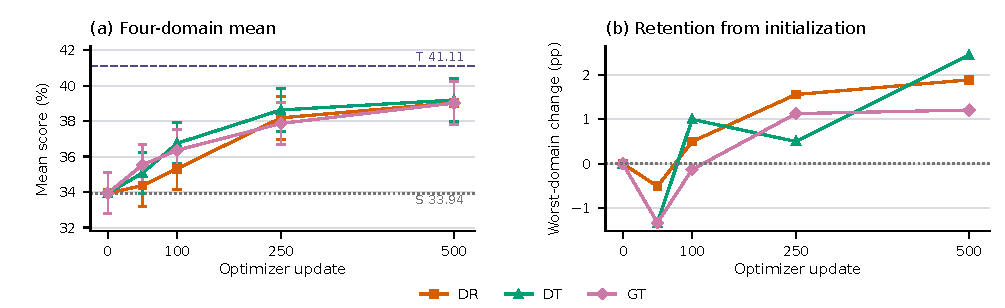
\includegraphics[width=\linewidth]{figures/table1_sync_20260918/section3_capability_support.pdf}
\caption{\textbf{Mean performance gains can coexist with a regression in an individual domain.}
(a) Four-domain mean $\pm$ std; S/T mark the initial student/teacher.
(b) Worst-domain change from initialization; zero means no regression. Lines connect reported point estimates.}
\label{fig:normalization_aggregate_support}
\end{figure}



\begin{figure}[t]
\centering
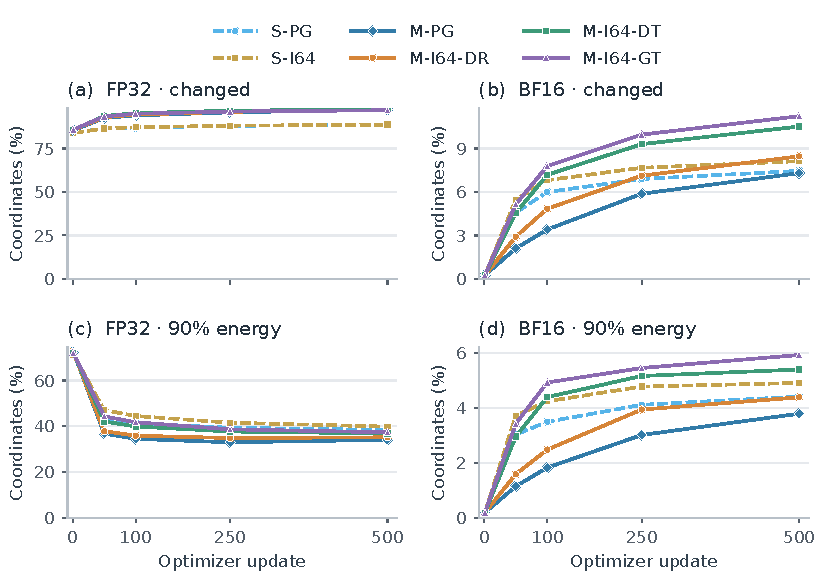
\includegraphics[width=\linewidth]{figures/visual_mvp_20260918/qwen_cumulative_geometry.pdf}
\caption{\textbf{Cumulative BF16 changes remain much sparser than FP32 changes.}
PG/I64 trajectories under DR in single-teacher (S) and joint (M) training, with joint I64-DT/GT added: (a,b) nonzero coordinate fractions; (c,d) coordinate fractions containing 90\% of squared displacement from initialization. Lines connect measured updates 1, 50, 100, 250, and 500; dashed lines denote S.}
\label{fig:geometry}
\end{figure}


\section{Completed Capability Comparisons and Additional Controls}
\label{app:completed_results}

\subsection{Evaluation scope and the independent domain test}
\label{app:independent_domain_test}

Table~\ref{tab:completed_endpoints} reports ten joint-training configurations at update 500, each using training seed 42. This matrix combines the previously reported PG-DR and I64-DR/DT/GT Adam trajectories with I16-DR, PG-DT/GT Adam, and PG-DR/DT/GT SGD. It does not represent ten additional runs beyond the earlier trajectories. The original benchmarks contain 500 mathematics questions, a 128-question LiveCodeBench slice, 300 IFBench questions, and 198 GPQA-Diamond questions. Mathematics, code, and IF use one response per question; GPQA uses four responses, averaged within question. The full development grid comprises 37 trained checkpoints and one shared initial evaluation: updates 50/100/250/500 for the seven Adam trajectories and 100/250/500 for the three SGD trajectories.

Table~\ref{tab:independent_test} uses a separately frozen additional-domain test with 256 questions per domain, for 1,024 questions and 1,792 responses per model. Mathematics and code are drawn from the Skywork-OR1-RL-Data mathematics and TACO-based code pools; IF uses Nemotron-RL-instruction\_following; Science uses the Nemotron-RL-knowledge-mcqa validation split restricted by a fixed natural-science keyword filter. Questions are the first eligible unique candidates in frozen source order, selected without model scores. Normalized exact and lexical near-duplicate checks exclude the original training bundle and known evaluation pools. These checks do not establish exhaustive semantic decontamination or absence of pretraining exposure.

The additional test uses math answer verification, code unit tests, instruction-following constraints, and science multiple-choice scoring. Mathematics, code, and IF use greedy decoding; Science uses four responses per question at temperature 1. The generation context budget is 32,768 tokens, with thinking disabled. The source distributions and the code/IF scorers differ from the original benchmark protocol, so the two tables are reported separately. All completed code evaluations have zero recorded infrastructure errors. The four-domain mean is an equal-weight descriptive aggregate. The available question-paired bootstrap intervals describe finite-test uncertainty, not variability across independent training seeds.

% Generated by export.py from data.json; do not edit numbers.
\begin{table}[t]
\centering
\small
\setlength{\tabcolsep}{5pt}
\caption{Independent additional-domain test scores (percent). Each domain has 256 questions; Science averages four responses per question. This test uses different source distributions from the original benchmarks. Update 250 for PG-DT / Adam is included because both frozen selection rules chose it. All trained models use seed 42; Mean is the unweighted domain average.}
\label{tab:independent_test}
\begin{tabular}{lrrrrrr}
\toprule
Configuration & Update & Math & Code & IF & Science & Mean \\
\midrule
Initial student & 0 & 42.97 & 23.44 & 25.78 & 62.21 & 38.60 \\
PG-DR / Adam & 500 & 46.48 & 26.17 & 37.50 & 64.06 & 43.55 \\
PG-DT / Adam & 250 & 44.53 & 26.56 & 36.72 & 64.75 & 43.14 \\
PG-DT / Adam & 500 & 44.92 & 27.34 & 38.28 & 63.48 & 43.51 \\
PG-GT / Adam & 500 & 44.92 & 28.91 & 39.06 & 65.14 & 44.51 \\
I16-DR / Adam & 500 & 44.92 & 28.52 & 40.23 & 64.55 & 44.56 \\
I64-DR / Adam & 500 & 46.88 & 26.17 & 39.06 & 65.72 & 44.46 \\
I64-DT / Adam & 500 & 43.36 & 27.73 & 39.06 & 64.55 & 43.68 \\
I64-GT / Adam & 500 & 45.31 & 27.34 & 41.02 & 66.21 & 44.97 \\
PG-DR / SGD & 500 & 46.88 & 27.73 & 37.11 & 62.21 & 43.48 \\
PG-DT / SGD & 500 & 46.48 & 28.52 & 37.11 & 63.48 & 43.90 \\
PG-GT / SGD & 500 & 44.53 & 26.17 & 36.72 & 64.45 & 42.97 \\
\bottomrule
\end{tabular}
\end{table}


\subsection{Frozen checkpoint-selection outcomes}
\label{app:completed_selection}

The selection protocol fixes a tolerance of 2 percentage points per domain relative to initialization, equal domain weights, and a minimum useful mean gain of 1 percentage point. It compares the endpoint, maximum-development-utility checkpoint, and maximum-utility checkpoint satisfying the retention constraints. Selections were frozen before the selected models' independent test inference. Development selection uses the already observed original benchmarks and is therefore exploratory.

% Generated by export.py from data.json; do not edit numbers.
\begin{table}[t]
\centering
\small
\setlength{\tabcolsep}{5pt}
\caption{Frozen checkpoint choices. Max utility and retention select the same checkpoint in every trajectory. Test $\Delta$ is the selected-checkpoint mean minus the endpoint mean in percentage points.}
\label{tab:checkpoint_selection}
\begin{tabular}{lrrrr}
\toprule
Trajectory & Endpoint & Max utility & Retention & Test $\Delta$ (pp) \\
\midrule
Other nine trajectories & 500 & 500 & 500 & 0.000 \\
PG-DT / Adam & 500 & 250 & 250 & -0.366 \\
\bottomrule
\end{tabular}
\end{table}


The retention and maximum-utility rules select identical checkpoints in all ten trajectories. Nine trajectories select update 500 under all three rules. For PG-DT/Adam, the two selection rules choose update 250: its independent-test mean is 43.140\%, compared with 43.506\% at update 500. Thus this comparison does not establish an advantage for retention-constrained selection. All selected models satisfy the retention and useful-gain conditions as test point estimates; this is not a simultaneous confidence guarantee. PG-DR/Adam has two development checkpoints outside the tolerance: GPQA falls from 32.197\% initially to 28.030\% at update 50 and 30.177\% at update 250, before reaching 34.975\% at update 500. Endpoint retention therefore does not imply retention throughout training.

\subsection{Actual intersection coverage}
\label{app:actual_intersection_coverage}

% Generated by export.py from data.json; do not edit numbers.
\begin{table}[t]
\centering
\footnotesize
\setlength{\tabcolsep}{5pt}
\caption{I64 candidate intersections retain high student probability mass. Mass is in percent; means and minima are over sampled prefixes. $r=p_\theta(I\mid h)/p_\theta(S\mid h)$ is the retained weight ratio.}
\label{tab:intersection_coverage}
\begin{tabular}{lrrrrrr}
\toprule
Student state & $p(I)$: mean & $p(I)$: min & $|I|$: mean & $|I|$: min & $r$: mean & $r$: min \\
\midrule
M-PG/100 & 99.9141 & 96.5482 & 58.96 & 43 & 0.9999413 & 0.9977714 \\
M-PG/500 & 99.9952 & 99.7825 & 61.59 & 50 & 0.9999975 & 0.9998511 \\
M-I64-DR/100 & 99.9564 & 97.5664 & 60.08 & 36 & 0.9997331 & 0.9757993 \\
M-I64-DR/500 & 99.9826 & 99.3722 & 61.75 & 51 & 0.9999912 & 0.9997005 \\
\bottomrule
\end{tabular}
\end{table}


Table~\ref{tab:intersection_coverage} measures the student probability mass in the actual student--teacher candidate intersection, rather than in the teacher candidate set alone. All 384 sampled routed prefixes have intersection mass above 95\%, and none has an empty intersection. This high-coverage regime helps delimit the local comparisons with full-vocabulary feedback. It does not establish the same behavior for low-coverage prefixes, other teacher configurations, or the full online I16 training trajectory. The four banks are local sampling repeats, not independent training seeds; inputs can differ across student states.

\subsection{Sensitivity to known mathematics overlap}
\label{app:math_overlap_sensitivity}

The frozen Qwen training pool contains five records matching four known MATH-500 underlying problems, including wording or answer-form variants. The affected MATH test identifiers are counting-and-probability problem 430 and intermediate-algebra problems 1849, 2146, and 582. Their presence in the training pool does not establish that each was sampled by a particular run or caused a performance increase. We remove these four fixed evaluation questions from the existing per-question scores as an offline sensitivity analysis, retaining the original 500-question results as the main protocol.

% MATH subset scores retained; means synchronized with the authoritative Table 1 domain scores.
\begin{table}[t]
\centering
\small
\setlength{\tabcolsep}{5pt}
\caption{\textbf{Removing four overlapping mathematics questions can reorder near-tied configurations.} Mean (496) substitutes MATH-496 for MATH-500 and keeps the other domain scores fixed.}
\label{tab:math496_sensitivity}
\begin{tabular}{lrrrrr}
\toprule
Configuration & Update & MATH-500 & MATH-496 & Mean (500) & Mean (496) \\
\midrule
Initial student & 0 & 68.80 & 69.15 & 33.94 & 34.02 \\
PG-DR / Adam & 500 & 73.20 & 73.79 & 38.61 & 38.76 \\
PG-DT / Adam & 250 & 77.00 & 77.42 & 38.78 & 38.89 \\
PG-DT / Adam & 500 & 73.20 & 73.59 & 38.60 & 38.70 \\
PG-GT / Adam & 500 & 76.20 & 76.81 & 38.60 & 38.75 \\
I16-DR / Adam & 500 & 75.40 & 76.01 & 38.90 & 39.06 \\
I64-DR / Adam & 500 & 75.80 & 76.41 & 39.04 & 39.19 \\
I64-DT / Adam & 500 & 74.00 & 74.40 & 39.19 & 39.29 \\
I64-GT / Adam & 500 & 74.20 & 74.60 & 39.02 & 39.12 \\
PG-DR / SGD & 500 & 76.40 & 77.02 & 39.96 & 40.12 \\
PG-DT / SGD & 500 & 75.20 & 75.81 & 39.44 & 39.59 \\
PG-GT / SGD & 500 & 75.00 & 75.60 & 38.58 & 38.73 \\
\bottomrule
\end{tabular}
\end{table}


The ordering by four-domain mean is unchanged across the twelve reported checkpoints. The frozen checkpoint selections are retained. This comparison neither retrains on a filtered pool nor constitutes an exhaustive overlap or contamination audit.

\subsection{Teacher-update overlap and distributional similarity}
\label{app:teacher_overlap_support}

\begin{figure}[t]
\centering
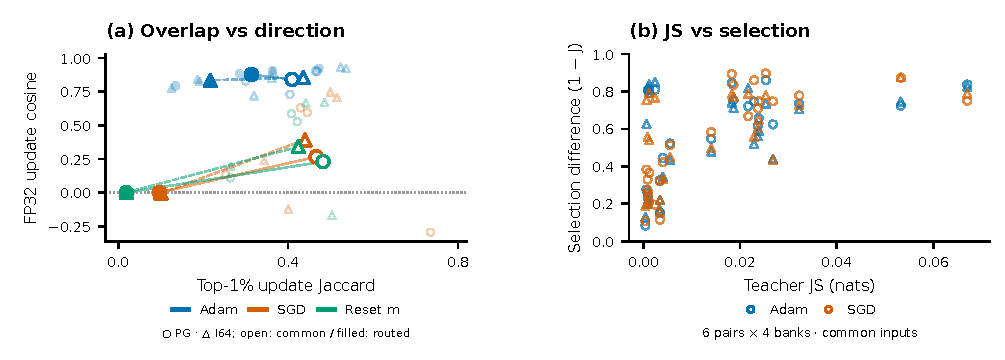
\includegraphics[width=\linewidth]{figures/nine_panel_20260914/appendix_teacher_overlap.pdf}
\caption{Supporting overlap views at the shared M-PG/500 student and optimizer state. (a) Top-1\% FP32 update-set Jaccard versus update cosine for PG/I64, common/routed inputs, and saved-state Adam, reset-$m$, and norm-matched SGD. Small points summarize banks and large points average four banks. (b) Common-input teacher JS versus $1-$Jaccard for Adam and SGD; each point is one teacher pair within one bank (six pairs per bank, four banks). Pairs share teachers and banks, so these points are dependent. These geometric associations do not measure cross-domain capability harm.}
\label{fig:teacher_overlap_support}
\end{figure}

Figure~\ref{fig:teacher_overlap_support} preserves the overlap and teacher-distribution comparisons alongside the history-subtracted controls in the main text. It uses local updates on copies of a saved state, not bitwise replay of the online optimizer. Common inputs hold the student prefixes fixed across teachers; routed inputs change the teacher and its input domain together.

\section{SmolLM3 Diagnostics and Capability Evaluation}
\label{app:smollm_diagnostics}

\subsection{Checkpoints, responses, and weighting}

We use the SmolLM3-3B MixSFT student, three domain-specific RL teachers, and exported 500-update students for I64-DR/DT/GT and PG-DR/SGD. The model and data revisions, export hashes, and diagnostic source snapshots are recorded with the measurements. The reported I64 training configurations use Adam with learning rate $2.5\times10^{-7}$; PG uses SGD with learning rate $0.0025$. The capability comparison uses a new shared evaluation protocol.

Diagnostic prompts come from the frozen Open-MOPD data revision \texttt{9e897efe}, with unique raw messages shuffled within mathematics, code, and instruction following. Coverage, normalization, and probe prompt splits are disjoint within this diagnostic sample. We preserve dataset messages and disable thinking in the chat template. Generation uses temperature 1, top-$p=1$, a 2,048-token prompt cap, and a 4,096-token response cap. Each natural coverage bank contains 384 responses, 128 per domain, with up to eight uniformly spaced positions per response: 3,053 prefixes for MixSFT and 3,058 for DR500. Additional students score the same 3,058 DR500 prefixes without regenerating responses.

Coverage statistics assign equal weight to domains, responses within domains, and audited positions within a response. Mean-mass intervals resample responses independently within each domain 2,000 times using seed 1042/1043/1044. MixSFT and DR500 use their own natural banks; the remaining students use the DR500 bank. The minimum I64 mass on DR500's natural bank is $1.7\times10^{-8}$; DT500 and GT500 each have one empty intersection in the common-bank audit.

\subsection{Frozen subsets and gradient comparisons}

Within each domain we select representative prefixes, prefixes above its 75th entropy percentile, and prefixes with I64 mass below 0.99. Selection allows overlap between strata and uses up to 32 distinct prompts per domain. The low-coverage code stratum has 21 eligible prompts, yielding 85 distinct prefixes overall. Each stratum is divided into three batches. Small candidate budgets $k=4,8$ are selected by a coverage-only rule.

The BF16 coverage audit sorts a top-128 list and takes its first $k$ entries, whereas gradient diagnostics recompute top-$k$ directly in FP32 at the exported BF16 parameter values. Student forward/backward passes use FP32; cached teacher targets use BF16 forward passes followed by FP32 log-softmax. One of the 85 frozen low-coverage prefixes crosses 0.99 during the FP32 diagnostic and remains in its original stratum. The FP32 diagnostic mean I64 masses are 99.05\%, 95.68\%, and 93.12\% for the representative, high-entropy, and low-coverage groups.

Full KL, PG, and intersection objectives use the definitions in Appendix~\ref{app:losses}. Empty intersections produce zero loss. We retain zero- and small-norm cases and report vector differences in addition to cosine. The plotted relative error is $\|g_{I_k}-g_{\mathrm{full}}\|/\|g_{\mathrm{full}}\|$, which measures the vector difference relative to the full-vocabulary gradient norm.


\subsection{Cumulative BF16 changes by parameter group}

The exported MixSFT-to-DR500 comparison contains 3,075,098,624 unique parameter coordinates after accounting for tied embeddings. The 36 transformer blocks each contain 78,123,008 coordinates, the token embedding 262,668,288, and the final normalization 2,048. We compare the two BF16 exports directly. Overall, 10.47\% of coordinates change; the largest 1\% carry 36.85\% of squared displacement, and 5.85\% of coordinates carry 90\%. Figure~\ref{fig:smollm_cumulative} retains all parameter groups. Per-group changed fractions use each group's own coordinate count; displacement shares use total model squared displacement.

\begin{figure}[p]
\centering
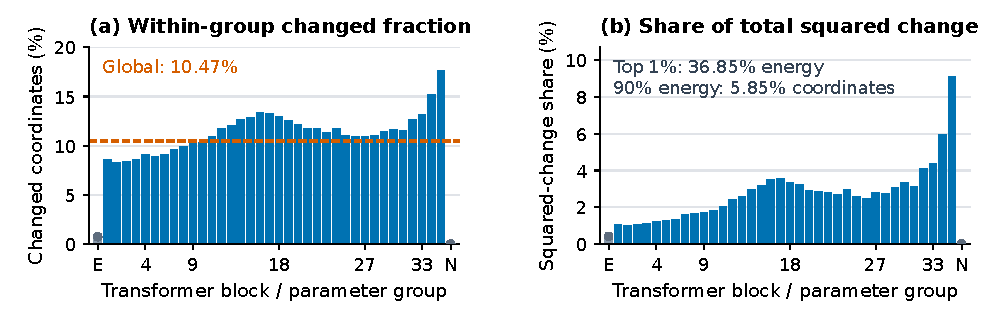
\includegraphics[width=\linewidth]{figures/visual_mvp_20260918/smollm_cumulative.pdf}
\caption{\textbf{Cumulative BF16 changes differ across all 38 SmolLM3 parameter groups.}
MixSFT to DR500: blocks 0--35, embedding (E), final norm (N). (a) Within-group changed fraction; dashed: global parameter-weighted fraction. (b) Share of total squared displacement. Tied weights count once.}
\label{fig:smollm_cumulative}
\end{figure}



\end{document}
